\documentclass[11pt]{article}

% ===== Packages =====
\usepackage[margin=1in]{geometry}
\usepackage{amsmath, amssymb}
\usepackage{graphicx}
\graphicspath{{../figures/}{figures/}{}}
\usepackage{booktabs}
\usepackage{siunitx}
\usepackage[hidelinks]{hyperref}
\usepackage{microtype}
\usepackage{setspace}
\usepackage{caption}
\captionsetup{font=small, labelfont=bf}

\title{\bfseries The Physical Riverbed Hypothesis:\\ Structural Boundaries and Cross-Hardware Validation of an Embodied Evolution System under Extreme Constraints}

\author{Author Name \thanks{Corresponding author.} \\
  \small Department, Institution, City, Postal Code, Country}
\date{}

\begin{document}

\maketitle

\begin{abstract}
\noindent
The core tenet of embodied intelligence holds that intelligence emerges from the coupling among a body, its environment, and simple control laws, yet the deeper question of \emph{to what extent the physical structure itself acts as an algorithm} has long lacked an operationally testable formulation. This paper reports an embodied evolution system completed under extreme resource constraints (three months, a single developer, no off-the-shelf platform): an obstacle-escape robot driven by novelty search and deployed on two heterogeneous ESP32 hardware platforms. Under the ``no-calibration, no-filtering, no-PID'' principles, the system consumes hardware thermal noise as its input and relies on a structure-first data pipeline (magic-number validation, fixed-width delta compression, CRC32 checksums, and atomic writes) to enable remote recomputation of process data. The analysis adopts self-controlled differencing and MAD-robust cleaning, taking the non-triggering of pre-registered falsification conditions as the acceptance criterion. Based on nine baseline datasets spanning 20+ generations and one heterogeneous-hardware dataset spanning 10 generations, three conclusions emerge. First, structural signatures---novelty that rises then plateaus, a non-degenerating rule count, and chaos constrained to left-wheel deceleration---reproduce stably across hardware and firmware versions, supporting the main conjecture. Second, the weak-version hypothesis (that specific sensor parameters directly determine specific behaviors) is rejected as a Simpson pseudo-correlation once environmental confounds are removed; physical structure therefore acts not as a rigid rope that directly drives behavior, but as a \emph{physical riverbed} that constrains the parameter-evolution space through epistatic effects. Third, when the perceptual information bandwidth is degraded and the noise-source pin is polluted by on-chip Flash multiplexing, the algorithm retains basic diversity, yet capability-side metrics (speed, survival, and the four-class criteria) become non-computable owing to acquisition defects. The paper thereby delineates the applicable boundary of the physical riverbed hypothesis and argues that data provenance is the only bridge capable of turning process-state data into scientific evidence.
\end{abstract}

\noindent\textbf{Keywords:} embodied intelligence; evolutionary robotics; novelty search; physical riverbed hypothesis; data provenance; structural boundary

\section{Introduction}
\label{sec:intro}

The fundamental claim that distinguishes embodied intelligence from the symbolic-computation tradition is that intelligence cannot be studied in isolation from the body that carries it and the environment in which it is situated. Brooks, in his ``intelligence without representation'' program, pointed out that complex behavior can emerge naturally from the coupling of a body, an environment, and simple control laws \cite{brooks1991}. Evolutionary robotics takes this further by automatically searching for controllers through evolutionary algorithms, among which novelty search is representative of open-ended evolution because it does not rely on an explicit objective function and instead rewards behavioral diversity \cite{lehman2011}.

However, a large portion of this literature still treats the physical body as a passive vehicle ``driven'' by the algorithm, implicitly assuming that the algorithm determines everything. What this paper tests, rather, is the affirmative thesis and its boundary in the opposite direction---what we term the \emph{physical riverbed hypothesis}: whether the body (its differential-drive geometry, sensor mounting, motor asymmetry, and noise-source purity) is not passive after all, but constrains and even shapes the trajectory of behavioral evolution at a deep level. It is worth stressing that this work originated from the metaphor of ``physical structure as algorithm''; after data-driven falsification it has been restated precisely as the testable \emph{physical riverbed hypothesis}. The rigorous verification of such a conjecture is usually carried out in a standard laboratory, on controlled hardware, and under a fixed software version. The distinctive feature of the present work is that the system was born from a three-month, single-developer engineering cycle in which the hardware underwent heterogeneous reconstruction from configuration A to configuration B, a filesystem migration, and several firmware jumps.

Upon methodological re-examination, this apparent ``disadvantage'' becomes a \emph{natural variation test}. If behavior were dominated by code logic, then the drastic firmware revisions would necessarily scatter the evolutionary trajectory; conversely, if data spanning different firmware and hardware forms still converge to the same macroscopic behavioral patterns, this constitutes the strongest empirical evidence for the physical riverbed hypothesis. The contributions of this paper are fourfold:

\begin{itemize}
  \item A structure-first data pipeline design (Section~\ref{sec:method}) that confers remotely-recomputable, traceable physical grounding on process data generated while the hardware was still un-frozen;
  \item An analysis protocol centered on ``self-controlled differencing + non-triggering of falsification conditions + robust cleaning'' (Section~\ref{sec:protocol}) that turns process data into conclusions usable for falsification;
  \item A cross-hardware, cross-firmware consistency test of structural signatures (Section~\ref{sec:results}), and the structural boundary it delimits;
  \item An honest registry of negative results and a deletion list (Sections~\ref{sec:results} and~\ref{sec:discussion}) that contracts the claim from a ``strong conjecture'' to a ``structural boundary,'' clarifying that the evolutionary lever resides in the algorithm-parameter layer while the fulcrum is supplied by the physical structure.
\end{itemize}

\section{Methodology: Hardware and Data Infrastructure}
\label{sec:method}

We first describe the minimal hardware platform under extreme constraints, then argue why a ``structure-first data pipeline'' is a precondition for this study, and finally delineate the platform boundary through hardware heterogeneity and a post-hoc audit of the GPIO conflict.

\subsection{A Minimal Hardware Platform under Extreme Constraints}
This study did not begin in a complete laboratory environment but in a three-month, single-developer engineering cycle. To verify the boundary that physical structure imposes on evolutionary behavior, we constructed two deliberately differentiated minimal platforms, configuration A and configuration B.

Both platforms follow the ``three-no'' principle---no calibration, no filtering, no PID---which severs external algorithmic compensation and feeds hardware thermal noise directly into the system. Configuration A (the baseline) is based on the ESP32-M-4M with a Sharp infrared ranging sensor (GP2Y0A21YK0F) whose output is a continuous analog signal, preserving gradient quantification of the environmental stimulus. Configuration B (the extended comparison) is based on the ESP32-N16R8 (16 MB Flash + 8 MB PSRAM) with a TCRT5000 reflective sensor, which, although also analog in output, is strongly affected by environmental reflectance and mounting geometry and therefore exhibits markedly lower signal-to-noise ratio. The two platforms differ not only in pin topology but also in \emph{perceptual information bandwidth} and \emph{noise-source purity}, forming a strict controlled-variable contrast.

\subsection{A Structure-First Data Pipeline and Audit Contract}
During a rapid iteration period in which neither hardware nor firmware was frozen, conventional plain-text logs are easily rendered unreadable by struct changes. To avoid this, the system enforces a strict structure-first data pipeline at the lowest level.

Every in-memory struct (e.g., \texttt{FrameLogEntry}, \texttt{BehaviorRule}) must be declared \verb|__attribute__((packed))| before being written to disk and then undergoes variable-length serialization and delta compression (e.g., the 11-byte fixed-width compression of frame logs). Each binary file mandatorily carries a 4-byte magic number, a version field, and a CRC32 checksum; writes use a two-stage atomic scheme (``temporary file $\rightarrow$ verify $\rightarrow$ rename'').

The core value of this engineering contract is that even in a ``process state'' of drastic firmware revision, all historical binary data retain a physical basis for off-site recomputation and traceability. This is the precondition that allows the present study to convert ``process data'' into scientific evidence.

\subsection{Protocol Freezing and Data Provenance}
Because the data contain extensive platform-construction trial-and-error, a formal protocol-freezing node was established: the EXSIMP version dated September 16 was fixed as the terminal data-pipeline convention. This version introduced the EXSIMP (Extreme Simplification of Persistence) storage policy and eliminated the directory-pressure deadlock that had previously frozen generation 10.

For pre-freeze data, provenance isolation is enforced through firmware pin assignment (e.g., GPIO4/5 vs.\ GPIO1/2) and file-header metadata. To address the lag of parsing scripts after data had been written (e.g., a parsing constant \texttt{SIZE\_COMPRESSED\_FRAME}=12 misaligning with the firmware's actual 11 bytes), the analysis stage introduced a data-auditing mechanism that forces a correction of the parsing offset through a length-closed hard check (e.g., $24 + 11 \times \texttt{frameCount}$), ensuring absolute consistency of the analysis convention across the nine firmware-version datasets. All core conclusions reported here are based on recomputed results after stride correction.

\subsection{Hardware Heterogeneity and Physical Information Bandwidth}
The platform of this study was not finalized in one step but evolved through ``trial assembly $\rightarrow$ final adoption.'' To verify the universality of the algorithm and the boundary of physical structure, we constructed configuration A (baseline) and configuration B (extended), whose chip-storage topology, peripheral pin assignment, sensor model, and mounting geometry constitute a strict physical heterogeneity, as summarized in Table~\ref{tab:hw}.

\begin{table}[!t]
\centering
\small
\caption{Physical and control-variable contrast between the two embodied hardware platforms.}
\label{tab:hw}
\begin{tabular}{@{}p{0.16\textwidth}p{0.26\textwidth}p{0.27\textwidth}p{0.24\textwidth}@{}}
\toprule
\textbf{Dimension} & \textbf{Config A (baseline EXSIMP)} & \textbf{Config B (extended N16R8)} & \textbf{Physical/algor. impact} \\
\midrule
MCU & ESP32-S3-M-4M (4 MB Flash) & ESP32-S3-N16R8 (16 MB Flash + 8 MB PSRAM) & B has more storage, enabling longer runs. \\
Filesystem & SPIFFS (EXSIMP) & FFat (later) & Late migration introduces mount-compatibility issues. \\
Sensor & Sharp GP2Y0A21YK0F & TCRT5000 reflective (AO analog out) & Sharp yields high-resolution continuous analog; TCRT5000 is low-SNR, degrading bandwidth. \\
IR pins & L: GPIO4 (ADC1\_CH3) / R: GPIO5 (ADC1\_CH4) & L: GPIO1 (ADC1\_CH0) / R: GPIO2 (ADC1\_CH1) & Both use ADC1 to avoid Wi-Fi; pin maps differ entirely. \\
Motor / encoder & PWM/DIR: 9/46, 16/15; Enc: 18/17, 11/10 & PWM/DIR: 17/18, 12/13/14/15 (L298N); Enc: 21/38, 4/5 & Re-pinning changes drive timing and encoder interrupt rate. \\
Noise pin (key) & GPIO6 (independent, floating) & GPIO6 (occupied by internal Flash on N16R8) & B's ``floating-noise'' mechanism may fail or read Flash-access noise. \\
Mechanics & 11 cm wheelbase, compact & breadboard chassis, all DuPont wires, low mount & B is asymmetric with higher supply ripple and EMI. \\
\bottomrule
\end{tabular}
\end{table}

From the ``information bandwidth'' viewpoint, configuration A provides high-dimensional continuous perceptual input, whereas configuration B is simultaneously degraded in signal-to-noise ratio and in noise-source purity. This control variable allows the subsequent experiments to directly test whether novelty search compensates for hardware defects under a low-bandwidth, noise-polluted physical structure (H-B) or leads to early exhaustion of the behavioral space (H-A).

Regarding engineering robustness, configuration B uses an all-DuPont-wire breadboard chassis and underwent a destructive filesystem migration from SPIFFS to FFat. Under power-drop and supply-ripple interference, such connections readily trigger mount failures; yet because the firmware strictly enforces a DATA-PRESERVED (anti-accidental-deletion) policy and two-stage atomic commit, the underlying binary experimental data remained intact even under crashes induced by the filesystem upgrade, confirming the survivability of the structure-first pipeline in extreme environments.

\subsection{Hardware Topology Constraints and GPIO Conflict: Post-hoc Hardware Audit}
\label{sec:audit}
Configuration B uses the ESP32-S3-N16R8. According to the official datasheet, GPIO6--8 are wired to internal Flash/PSRAM and cannot be used as general-purpose I/O. If the firmware still reads the noise source on that pin (\texttt{PIN\_NOISE\_SOURCE}=6), what it reads may not be semi\-conductor thermal noise but electromagnetic coupling noise during Flash bus access. Rather than trusting the documentation, this study infers the hardware state from data, implementing a post-hoc hardware audit.

Aggregating the \texttt{rawNoiseL}/\texttt{rawNoiseR} fields across all ten generations of chaos snapshots of configuration B (448 samples), the reading is not a constant dead value: its minimum is 0, maximum 423, mean 158.1, standard deviation 94.1, with 219 distinct values (zero-value ratio 0.67\%, top-value ratio only 1.8\%). But neither is it the full-scale, wide-range thermal noise expected of a clean floating ADC (12-bit full scale 0--4095, floating-thermal-noise expectation centered near $\approx$1800). The reading is stably clamped to the low band 0--423 with persistent small-amplitude fluctuation, as shown in Figure~\ref{fig:noise}.

\begin{figure}[!t]
\centering
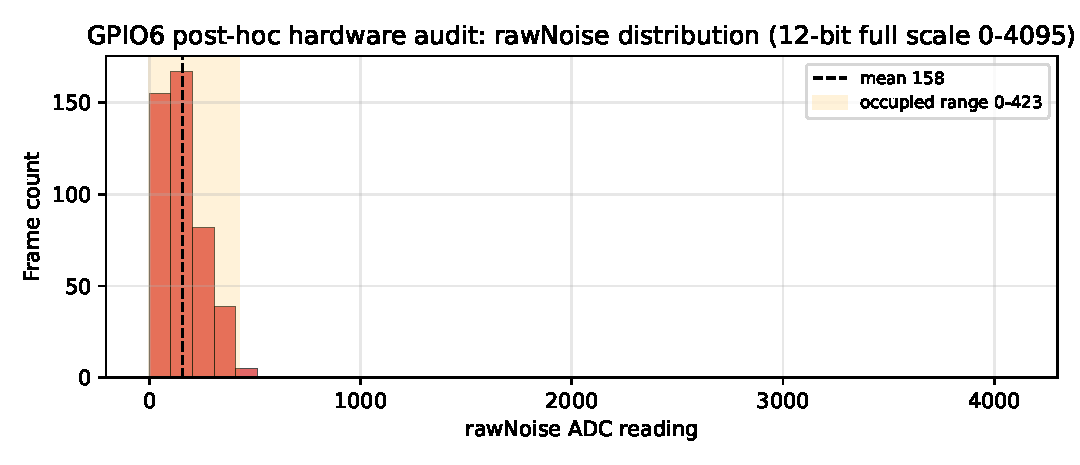
\includegraphics[width=0.72\textwidth]{fig_noise_hist.pdf}
\caption{Post-hoc hardware audit of GPIO6 on configuration B: distribution of rawNoise (full scale 0--4095).}
\label{fig:noise}
\end{figure}

This characteristic is highly consistent with the physical constraint that GPIO6 is multiplexed with internal Flash on the N16R8 module: the pin captures coupling noise from Flash access rather than independent semiconductor thermal noise, so the chaos randomness source is degraded at the physical layer into a ``low-amplitude pseudo-random source.'' Even so, it still provides non-zero random perturbation, so the chaos mechanism is not fully ``switched off''---a point that will be corroborated by the chaos-frame-ratio result in Section~\ref{sec:results}. This intermediate state of ``polluted but not deadlocked'' noise provides a valuable natural-experiment condition for studying the effect of noise-source purity on the diversity of open-ended evolution.

\section{Experimental Protocol and Falsification Logic}
\label{sec:protocol}

When the physical hardware is not yet fully finalized and the data contain extensive process noise, a traditional methodology based on independent significance testing between groups fails readily: ambient temperature drift, power ripple, DuPont-wire contact impedance, and firmware batch differences all directly swamp the evolutionary signal of the algorithm itself. This study therefore abandons frequentist significance testing in favor of a protocol combining ``self-controlled differencing'' with ``robust statistical cleaning,'' and anchors its core criterion on the \emph{non-triggering of falsifiable conditions}.

\subsection{Self-Controlled Experimental Design}
To eliminate hardware-batch, ambient-temporal, and individual intrinsic biases, this study introduces a self-controlled paradigm within a single continuous test.

Taking the physical-blocking instant $t^*$ that triggers the chaos intervention as the dividing line, one continuous test is split into two segments: the baseline (Baseline, $t < t^*$), representing the pure physical differential background, and the intervention (Intervention, $t \ge t^*$), representing the enhanced performance after physical noise takes over.

Because both segments come from the same hardware, the same ambient period, and the same mechanical inertial frame, all time-varying interference and hardware intrinsic bias automatically cancel in the within-individual difference ``intervention minus baseline.'' Four result classes A/B/C/D are thereby defined (e.g., $\Delta \text{distance} > 0$ and $\Delta \text{frames} > 0$ is class A, strongly supporting physical exploration; $\Delta \text{distance} < 0$ and $\Delta \text{frames} < 0$ is class D, strongly against). This design frees subsequent behavioral analysis from a standardized test arena.

\subsection{Unified Statistical Conventions and Robust Cleaning}
To compare across datasets, firmware revision makes individual initialization carry outliers from early instability. The offline statistical stage strictly enforces four principles (P1--P4) to align conventions:

\begin{itemize}
  \item P1 (per-generation mean): within a generation, indicators are averaged over individuals before cross-generation comparison, removing weight bias from anomalous population sizes.
  \item P2 (robust outlier removal): only for the novelty series, median absolute deviation (MAD) cleaning is applied ($|v - \text{median}| > 3.5 \times 1.4826 \times \text{MAD}$), removing initialization-instant extremes. This occurs purely offline and never smooths or denoises the raw sensor signal, strictly abiding by ``no filtering.''
  \item P3 (raw physical quantities): speed, distance, and variance are computed directly from the ratio or accumulation of raw PWM and encoder pulses, without physical-unit conversion (no calibration).
  \item P4 (no closed-loop intervention): all analysis is batch; no current observation is ever corrected by the previous generation's result (no PID).
\end{itemize}

\subsection{Falsification Logic and Negative-Result Auditing}
This study refuses to use the implicit fitness indicators of ``objective-directed optimization.'' To delimit the physical riverbed hypothesis, three falsification conditions were pre-registered (if triggered, the thesis is challenged):

\begin{itemize}
  \item F1: the novelty archive saturates shortly after the initial growth (early exhaustion of the exploration space);
  \item F2: the population's behavioral-descriptor dispersion decreases monotonically with generation (convergence to a single behavior);
  \item F3: the behavioral rule count degenerates to near-minimum and stops changing (loss of algorithmic capacity).
\end{itemize}

Across nine independent datasets spanning 20+ generations, none of the three conditions was triggered. Furthermore, to counter batch drift (the date effect) from firmware-version differences, a within-dataset demeaning test was applied. The result shows that the previously plausible weak hypothesis---that specific sensor parameters directly determine specific behaviors---is rejected as a Simpson pseudo-correlation once environmental confounds are stripped away, and that strong conjecture is explicitly falsified.

This paper commits to a public \emph{deletion list}: earlier single-dataset conclusions such as ``class A dominates'' (later shown to be class D domination) and ``coverage is positively correlated with rule count'' (later shown that coverage saturates early and lacks variance) are formally removed from the conclusion library because they failed cross-dataset reproduction.

\subsection{Behavior Invariance across Firmware Versions}
In a traditional controlled experiment, software and firmware iterations are typically treated as confounding variables to be tightly controlled. Yet during the three-month extreme development cycle of this study, the firmware underwent several major refactorings (including data-structure slimming, anti-deadlock-mechanism introduction, and a filesystem migration from SPIFFS to FFat), and the hardware also underwent pin reassignment and sensor replacement. If the system's behavior were dominated by code logic, these frequent iterations would necessarily cause drastic drift of the evolutionary trajectory.

However, analysis across the nine datasets (spanning old firmware and the frozen EXSIMP version) shows a strong logical internal consistency of the behavioral trajectory:
\begin{itemize}
  \item regardless of firmware version, novelty always shows a ``rise-then-plateau'' trend (the generation-1 mean is 3.0--7.6$\times$ the plateau);
  \item chaos-period behavior is always constrained to ``left-wheel deceleration'' ($P(\Delta L < 0) \ge 0.68$ in all nine datasets), unchanged by control-flow code updates;
  \item the behavioral library stably locks onto the ``turn--reverse'' complementary axis (correlation $-0.81$ to $-0.31$).
\end{itemize}

This constitutes strong empirical evidence for the physical riverbed hypothesis: software firmware is merely the carrier of the physical structure, while the evolutionary trajectory of macroscopic behavioral patterns is firmly anchored by the underlying physical structure (differential-drive geometry, motor asymmetry, sensor mounting). The continuous firmware iteration instead acts as a ``variation test'' of the physical structure, proving the stability of physical constraints at the cross-implementation level.

\section{Results}
\label{sec:results}

This section reports results based on nine independent datasets (baseline convention EXSIMP, 20+ generations) and the extended hardware platform (configuration B, N16R8 + TCRT5000, 10 generations). All conclusions are anchored on cross-dataset directional consistency and the non-triggering of falsification conditions.

\subsection{Baseline Platform (Config A): Behavioral Patterns and Structural Constraints}
Under the frozen EXSIMP convention, the system exhibits the following robust features within a 20-generation window:
\begin{itemize}
  \item Diversity maintenance and non-degenerating rule count: novelty peaks at generation 1 (1.60--3.38) and then stabilizes at the generation-11--20 plateau (0.39--0.60) in all nine datasets; the rule-count slope is $-0.062$ to $+0.246$ and never degenerates to the minimum, so falsification conditions F1 and F3 are not triggered.
  \item Physical anchoring of the behavioral library: across environments and firmware versions, chaotic-period behavior is constrained to ``left-wheel deceleration'' ($P(\Delta L<0) \ge 0.68$) and the ``turn--reverse'' complementary axis (correlation $-0.81$ to $-0.31$), confirming the enforcece of the physical differential structure.
  \item Speed--survival trade-off: at the individual level, movement speed and survival time are negatively correlated in all nine datasets (eight clearly negative, one near zero), indicating that exploratory motion carries a genuine physical cost priced by the hardware structure.
\end{itemize}

\subsection{Extended Platform (Config B): Physical Information Bandwidth Degradation and Hardware Conflict}
To verify the algorithm's robustness across physical forms, a 10-generation extended experiment was executed on configuration B (N16R8 + TCRT5000). Note that this platform suffered a filesystem (FFat) migration and a GPIO-reuse (GPIO6) conflict. The four measured aspects are as follows:
\begin{itemize}
  \item Post-hoc hardware audit (GPIO6): rawNoise readings fall in the low band 0--423 (mean 158.1, std 94.1), neither a constant dead value nor full-scale thermal noise; they constitute low-amplitude pseudo-random noise under Flash-reuse pollution (see Section~\ref{sec:audit}, Figure~\ref{fig:noise}).
  \item Behavioral characterization: configuration B's novelty likewise rises then plateaus---under MAD-robust convention the generation-1 median is 1.16 and the last-five-generation plateau mean is 0.27 (a ratio of $\approx$4.3$\times$; raw medians 3.76 $\rightarrow$ 0.26), identical in form to configuration A; the generation-10 mean rule count is 11.5 with a full-window mean of 8.3--14.3, never degenerating to the minimum of 2, so algorithmic capacity is retained.
  \item Chaos mechanism: the chaos frame ratio (chfr) has a full-window mean of 0.242 (per-generation 0.13--0.39), falling within configuration A's 0.16--0.46 band; chaos remains present and is not ``suffocated.''
  \item Acquisition-defect registry: \texttt{distance\_ticks} is uniformly 0 (encoder odometry produced no counts on N16R8) and \texttt{survival\_time} is capped at $\approx$25 s (25001--26238 ms); both make the speed convention, survival variance, and the A/B/C/D four-class differencing non-recomputable in this batch---an acquisition gap rather than a negated conclusion.
\end{itemize}

\begin{figure}[!t]
\centering
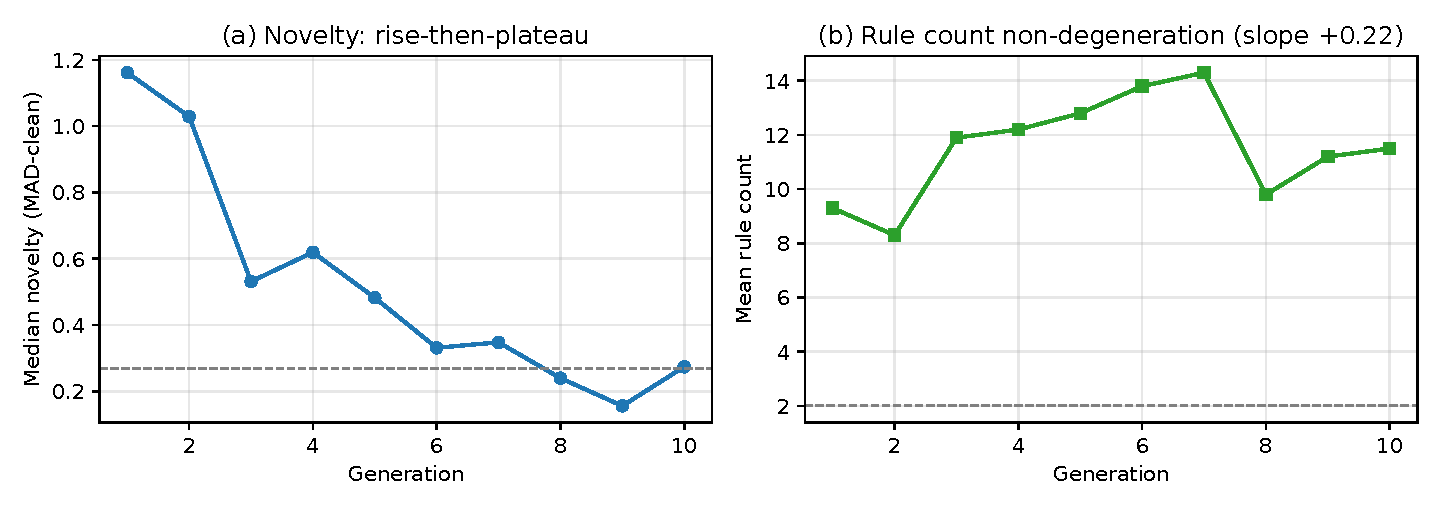
\includegraphics[width=0.75\textwidth]{fig_novelty_rules.pdf}
\caption{Configuration B: novelty ``rise-then-plateau'' and non-degenerating rule count.}
\label{fig:noveltyrules}
\end{figure}

\begin{figure}[!t]
\centering
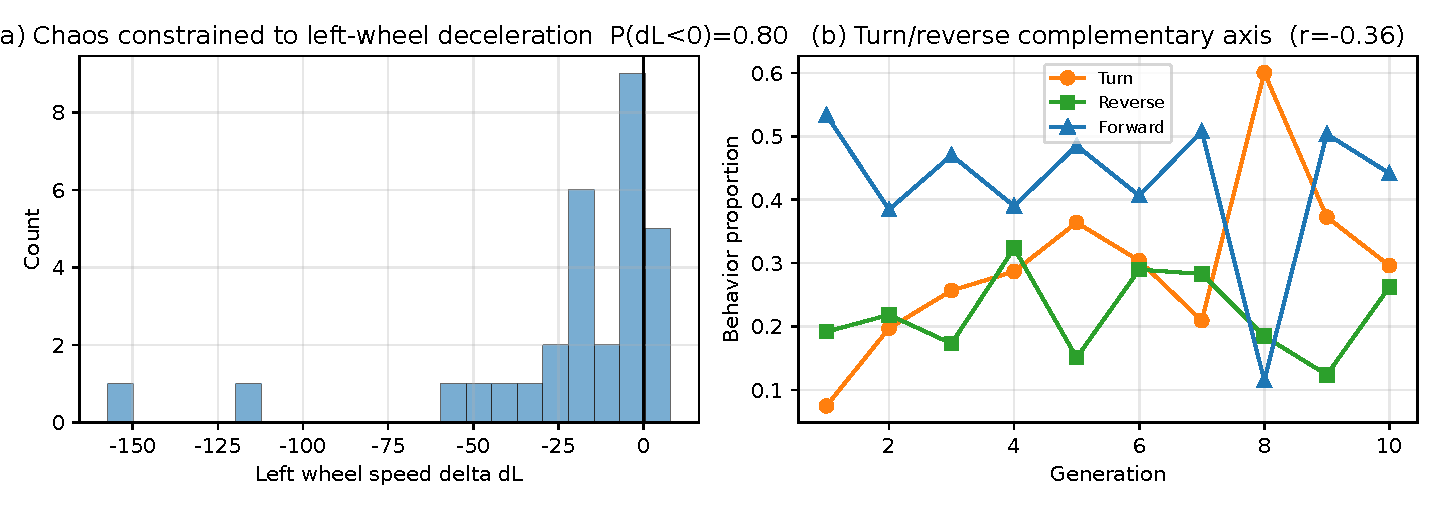
\includegraphics[width=0.75\textwidth]{fig_anchoring.pdf}
\caption{Configuration B: chaos anchoring behavior---left-wheel deceleration and the turn/reverse complementary axis.}
\label{fig:anchoring}
\end{figure}

\subsection{Cross-Platform Test of the Falsification Conditions}
The three falsification conditions were not triggered in configuration A; in configuration B (low information bandwidth, polluted noise source), conditions F2 (dispersion decrease) and F3 (rule-count degeneration) were likewise not triggered---although its physical information bandwidth was degraded and a GPIO-reuse conflict existed, the novelty series still maintained ``rise-then-plateau'' and the rule count remained above the non-degeneration threshold (generation 10: 11.5). This indicates that the variable-length gene and the novelty-search algorithm possess robustness across hardware-topology defects and can partially compensate for the missing information of the physical structure.

However, one important boundary must be registered simultaneously: the capability-side quantitative conclusions of configuration B (capability pricing of speed and survival, and the A/B/C/D four-class criteria) cannot be recomputed because encoder odometry is uniformly 0 and survival time is capped. Therefore the ``algorithmic robustness'' conclusion is, on configuration B, strictly limited to the structural-side signatures (novelty, rule count, chaos presence) and behavioral-side anchoring, and does not extend to the capability pricing that requires physical odometry and survival variance. This boundary itself hints that a low-bandwidth hardware, while not strangling diversity, does sever the observable channel of the speed--survival capability pricing.

\section{Discussion}
\label{sec:discussion}

This study completed an embodied-evolution experiment under extreme resource constraints yet did not arrive at a perfect ``paradigm''; rather, it arrived at a set of strictly delimited \emph{structural boundaries} and an honest \emph{falsification of a weak hypothesis}. Three points constitute the core insight.

\subsection{Physical Information Bandwidth Bounds Open-Ended Evolution}
Configuration A (high-resolution continuous analog) and configuration B (low-SNR reflective, coupled with the GPIO-reuse conflict of the N16R8) form a strict physical-bandwidth contrast. The results show that even under a low-bandwidth structure with a polluted noise source, novelty maintains ``rise-then-plateau'' and the rule count does not degenerate, indicating that the algorithm possesses a certain robustness; yet the capability-side observable channel (the speed--survival pricing) is severed by the absence of odometry and survival variance. This inversely indicates that the reason a ``no-calibration, no-filtering'' minimal physical structure can give rise to adaptive behavior is precisely that its sensors retain a high-dimensional information channel coupled to physical thermal noise. The physical riverbed hypothesis does not hold unconditionally; it is strictly bounded by the information bandwidth of the perceptual front end---once the structure can no longer supply sufficient physical gradients, the algorithm layer may maintain the \emph{form} of diversity but will lose the \emph{substance} of capability pricing.

A potential misunderstanding should be clarified here: since GPIO6 on configuration B is polluted by Flash multiplexing, has the chaos intervention lost its meaning? The answer is no. The proper duty of the chaos mechanism is not to supply statistically pure random numbers but to act as a \emph{symmetry-breaking} device at the moment of entrapment---the essence of a differential robot's deadlock is that the left and right wheel commands remain symmetric, and the point of chaos injection is precisely to impose an \emph{asymmetric} perturbation on the two sides to break the deadlock. Although the post-hoc audit found the GPIO6 reading clamped to the low band 0--423, it still exhibits 219 distinct values and the two channels are not equal ($\texttt{rawNoiseL} \ne \texttt{rawNoiseR}$), so it can still inject a non-zero asymmetric perturbation at the deadlock instant. The persistent presence of chaos frames in configuration B (chfr 0.242) and the stable constraint of chaos-period behavior to left-wheel deceleration ($P(\Delta L<0)=0.80$) are direct evidence that the mechanism still holds behavioral efficacy. What is degraded is not the \emph{meaning} of chaos but the \emph{quality} of the randomness source (its entropy and range): low-amplitude noise may be insufficient to inject a sufficiently strong perturbation in deep deadlock, and may carry predictable periodic patterns from Flash access, thereby weakening the diversity and efficiency of exploration. This distinction once again corroborates the core judgment of this paper---noise is only a symmetry-breaking trigger, and the true algorithm resides in the physical differential structure; so long as the structure survives, any left--right asymmetric perturbation will be projected into meaningful escape behavior.

\subsection{Data Provenance is the Only Bridge from Process Data to Scientific Evidence}
Evolutionary robotics has long faced a ``reproducibility crisis,'' and this is fatal during the rapid-iteration engineering development that this paper underwent (four firmware jumps and two filesystem migrations in three months). This study demonstrates that, before the hardware and protocol are frozen, by relying on a ``structure-first black box'' (magic numbers, fixed-width delta compression, CRC32, and atomic writes), the researcher can still retrospectively strip polluted process data into valid datasets usable for falsification. In particular, through firmware-version provenance (the September 16 EXSIMP protocol freeze) and the stride hard-check of the parsing script (11/12 bytes), we avoided the ``pseudo-emergence'' illusion caused by data misalignment. When the hardware is not yet finalized, the data pipeline itself is the most central scientific infrastructure.

\subsection{From a Strong Conjecture to a Structural Boundary}
In embodied intelligence, researchers often rush to propose grand ontologies. Yet the analysis of this paper, based on nine datasets spanning 20+ generations and using strict batch control (demeaning) and MAD-robust cleaning, yields a cold negative result: the previously plausible weak-version hypothesis that ``physical parameters directly determine behavior'' is rejected as a Simpson pseudo-correlation after removing environmental confounds.

This result should not be read as failure but as the core value of this study. It precisely delimits the domain of the physical riverbed hypothesis: physical structure does not directly determine behavior, but forms an \emph{epistatic effect} through algorithmic parameters (e.g., \texttt{stuckWindowSize}, \texttt{chaosTimeoutMs}). This contraction excludes the over-mystification of physical morphology and points out the direction for future work: the lever of evolution resides in the algorithm-parameter layer, but the fulcrum of the lever is supplied by the physical structure.

It is worth emphasizing that the falsification of the weak hypothesis (physical parameters do not directly determine behavior) and the invariance of macroscopic behavior (cross-firmware consistency) are not contradictory but form an important inverse indicator. If the system's behavior were dominated by code logic, the drastic firmware revision over three months would necessarily scatter the evolutionary trajectory; yet data spanning different firmware versions still stably lock onto the behavioral modes constrained by physical structure (e.g., the turn--reverse axis and left-wheel deceleration). This proves that physical structure does not play the role of a ``rigid rope'' directly driving behavior, but acts as a ``physical riverbed'': it constrains the parameter-evolution space through epistatic effects (S$\rightarrow$T robust), and the upper-layer evolution parameters ultimately realize specific behavior (T$\rightarrow$Y robust), while no direct mapping exists in the middle (S$\rightarrow$Y breaks). The weak version is falsified precisely because the mechanism of physical structure is indirect, epistatic, rather than mechanically deterministic.

It is worth noting explicitly that the earliest formalization attempt tried to characterize physical structure with a constrained manifold and a fiber, from which we derived the quantitative hypothesis H3 (that the ``evolutionary capacity'' correlates positively with evolutionary success, with novelty as the aligned criterion); in the data, H3 was not supported overall. The root cause of that failure is a category mismatch: the language of conservative systems (static geometry) cannot capture a novelty-driven dissipative system. The subsequent data reconstruction (cross-implementation behavioral invariance and the S$\rightarrow$T$\rightarrow$Y epistatic effect) then revealed the true mechanism of the physical structure: it is not a rigid ``rope'' but an elastic ``physical riverbed''---the macroscopic form of the water flow (behavior) is shaped indirectly by the river channel (structure), rather than being defined point by point.

\section{Limitations and Future Work}
This study honestly acknowledges the following limitations.

First, due to the extreme compression of the development cycle, the baseline data (EXSIMP frozen convention) amount to nine datasets spanning 20+ generations; the extended platform (configuration B) completed only a first round of 10 generations, and, owing to acquisition defects (uniformly-zero encoder odometry and capped survival), cannot support long-window capability-side evolutionary analysis.

Second, the strong-version geometric layer (real physical geometric quantities such as wheel track width and sensor mounting height) is not testable within this paradigm for lack of precise calibration data.

Third, after completing 10 generations of evolution, configuration B suffered mounting failures from the filesystem migration (FFat) and DuPont-wire connections; although the data were fully backed up, the longer-window evolutionary trend remains to be analyzed.

Future work will focus on four directions:

\begin{itemize}
  \item[(1)] Prototype scale-up and geometric-layer completion: on the frozen pipeline (EXSIMP), run 50--100 generations on both configurations; simultaneously collect precise chassis geometry to fill the empirical gap of the strong-version geometric layer, and repair encoder odometry and the survival threshold to restore capability-side recomputation.
  \item[(2)] Post-hoc audit of the GPIO6 noise source: perform detailed variance analysis of the GPIO6 polluted by N16R8 Flash reuse, delineate the destructive boundary of ``polluted physical noise'' on open-ended evolutionary diversity, or fly-wire the noise source to an independent ADC pin as a control.
  \item[(3)] Transplant validation at the algorithm layer: decouple the ``novelty-search + physical differential mapping'' module and deploy it onto ROS or more complex embodied forms, to examine its engineering feasibility as a ``low-power edge adaptive sub-brain.''
  \item[(4)] \textbf{Embodied Co-evolution: High-Dimensional Physical Reduction of Human Intent.} The validation of this paper is strictly confined to unsupervised autonomous evolution. Yet the higher-order form of embodied intelligence necessarily involves human--robot interaction. In traditional control paradigms, the human acts as an external observer or instruction issuer (e.g., sending target coordinates or preference feedback), which leaves a \emph{semantic gap} between human intent and the physical system. In future work, building on the verified ``physical riverbed'' mechanism, we will introduce \emph{high-dimensional tunable physical parameters} as the human--robot interface. Specifically, instead of issuing high-level commands through the algorithmic layer, the human adjusts physical boundary parameters such as sensor thresholds, thereby reducing and encoding human intent into a continuous modulation dimension of the evolutionary search space. This constitutes an \emph{embodied co-evolution} relationship: the human is no longer an issuing deity but becomes part of the universal physical structure, co-participating in physical evolution with the machine. Subsequent experiments will establish strict A/B comparisons (human-adjusted physical boundary parameters vs.\ traditional algorithmic preference feedback) to test whether this physical participation channel produces more concentrated and evolutionarily robust behavioral shifts.
\end{itemize}

\section{Conclusion}
This paper tested and delimited the physical riverbed hypothesis within an embodied evolution system under extreme constraints. The structural signatures (novelty rising then plateauing, non-degenerating rule count, chaotic left-wheel deceleration, and the turn--reverse complementary anchoring) reproduce stably across the cross-hardware, cross-firmware variation test, supporting the affirmative thesis that physical structure acts as a ``physical riverbed'' anchoring the behavioral evolutionary trajectory; the falsification of the weak-version hypothesis shows that the mechanism of physical structure is epistatic and indirect. The degradation of physical information bandwidth, while not strangling diversity, does sever the observable channel of capability pricing, thereby delimiting the applicable boundary of the conjecture. Throughout, the structure-first data pipeline is the fundamental premise that allows this series of conclusions to hold on the basis of ``process data'': before the hardware is finalized, data provenance is itself the most central scientific infrastructure.

In exploring embodied intelligence, the researcher is, in essence, himself a constrained physical structure. The movement of this study from an ontological conjecture to a mechanistic, falsifiable hypothesis records not only the evolutionary process of the robotic vehicle, but also an evolution completed by the research subject himself within the boundaries of physics and cognition.

\begin{thebibliography}{99}

\bibitem{brooks1991}
R.~A. Brooks, ``Intelligence without representation,'' \emph{Artificial Intelligence}, vol.~47, no.~1--3, pp.~139--159, 1991.

\bibitem{stanley2002}
K.~O. Stanley and R.~Miikkulainen, ``Evolving neural networks through augmenting topologies,'' \emph{Evolutionary Computation}, vol.~10, no.~2, pp.~99--127, 2002.

\bibitem{bongard2006}
J.~Bongard, V.~Zykov, and H.~Lipson, ``Resilient machines through continuous self-modeling,'' \emph{Science}, vol.~314, no.~5802, pp.~1118--1121, 2006.

\bibitem{lehman2011}
J.~Lehman and K.~O. Stanley, ``Abandoning objectives: Evolution through the search for novelty alone,'' \emph{Evolutionary Computation}, vol.~19, no.~2, pp.~189--223, 2011.

\bibitem{bongard2011}
J.~Bongard, ``Morphological change in machines accelerates the evolution of robust behavior,'' \emph{Proceedings of the National Academy of Sciences}, vol.~108, no.~4, pp.~1234--1239, 2011.

\bibitem{cully2015}
A.~Cully, J.~Clune, D.~Tarapore, and J.-B.~Mouret, ``Robots that can adapt like animals,'' \emph{Nature}, vol.~521, no.~7553, pp.~503--507, 2015.

\bibitem{doncieux2015}
S.~Doncieux, N.~Bredeche, J.-B.~Mouret, and A.~E.~Eiben, ``Evolutionary robotics: What, why, and where to,'' \emph{Frontiers in Robotics and AI}, vol.~2, p.~4, 2015.

\bibitem{mouret2015}
J.-B.~Mouret and J.~Clune, ``Illuminating search spaces by mapping elites,'' \emph{arXiv preprint arXiv:1504.04909}, 2015.

\end{thebibliography}

\end{document}